\documentclass[titlepage]{article}
\usepackage[utf8]{inputenc}
\usepackage{graphicx,wrapfig}
\graphicspath{{images/}}
\usepackage{amsmath}

\usepackage{geometry}
 \geometry{
 a4paper,
 total={170mm,257mm},
 left=20mm,
 top=20mm,
 }

\title{B1-report-Nihaar}
\author{nihaar shah }
\date{December 2016}

\begin{document}

\maketitle
%
\section{Introduction}
Every camera has intrinsic parameters that...
\subsection{Aim and Motivation}
To estimate and optimise the intrinsic parameters for a given set of extrinsic parameters of a camera that has been modelled roughly based on an iPhone 6 camera specifications.
%
Knowledge of intrinsic parameters is very useful to find real world distances of planar objects just from their images and if we know the position and orientation where our camera is mounted with respect to our images. By using multiple cameras (because multiple can provide depth information) this could also be used to do 3D reconstruction
%
\subsection{Camera Model Specifications}
We have used an ideal pinhole camera model excluding the effects of radial or tangential lens distortion as a simplification. The 8 intrinsic parameters are Chip Width and Height, Focal Length, Effective Width and Height of a pixel, Skewness, Principal point offsets in the x and y directions which are used to define the K-Matrix.
(Maybe later consider effects of changing these on the final estimation or optimisation?)
%
% The KMatrix equation 
\begin{equation} \label{KMatrix}
K=
  \begin{bmatrix}
  \alpha f & \gamma f & t_u \\ 
  0        & \beta f  & t_v \\ 
  0        &    0     &  1 
  \end{bmatrix}
\end{equation}
%
\subsection{Outline}
\subsubsection{Simulation}
%
\begin{figure}
\caption{Simulated cube in the camera's field of vision-a test of PositionCamera and PositionImage functions.}\label{wrap-fig:9}
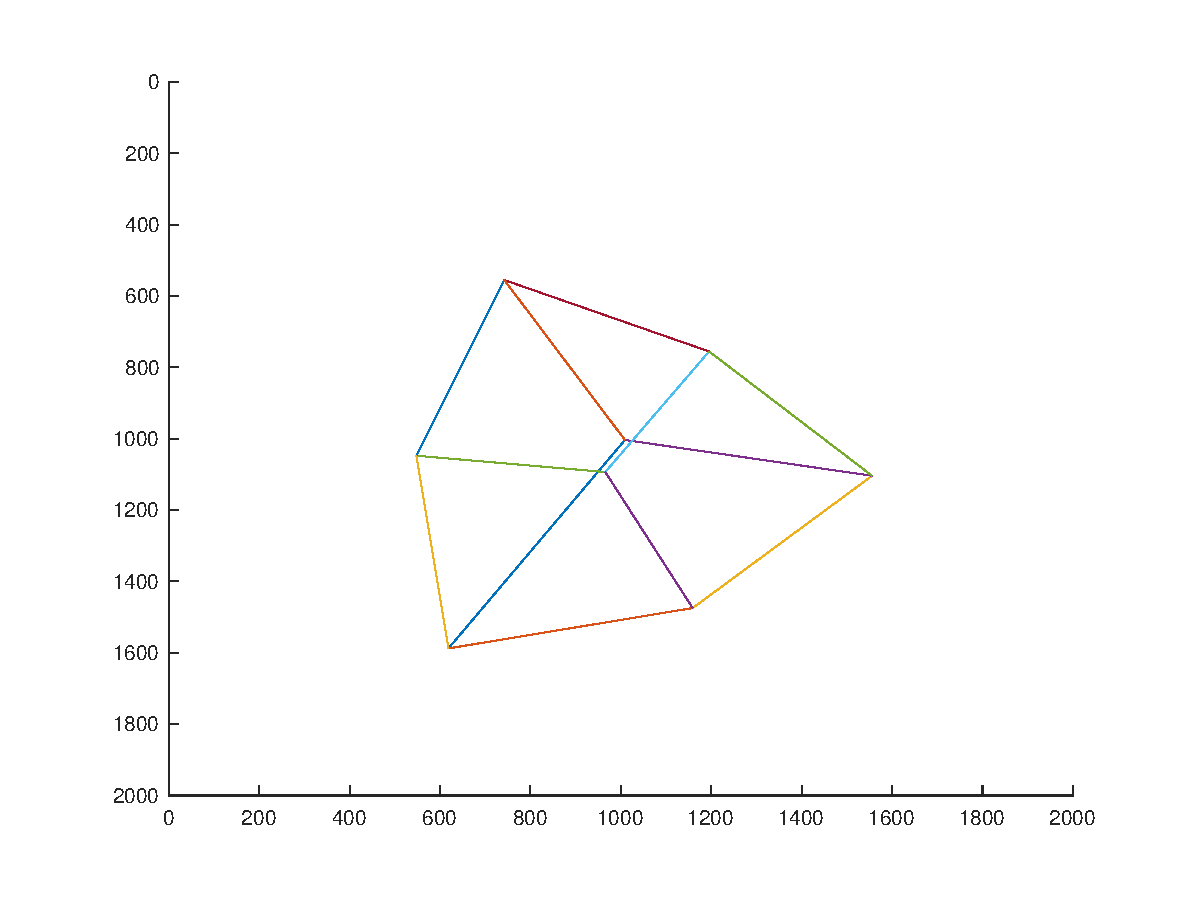
\includegraphics[width = 4.5cm, height=4.5cm]{SimulateCube.eps}
\end{figure}
4MP camera hence 2000 x 2000 dimensions of image.
%
\subsubsection{Initial Estimate}
% The object to image conversion equation 
\begin{equation}\label{uv-to-xy}
\begin{bmatrix}
  U\\ 
  V\\ 
  S 
  \end{bmatrix}
        = \textbf{K}
         \begin{bmatrix}
 \textbf{r1} & \textbf{r2} & \textbf{t}
         \end{bmatrix}
        \begin{bmatrix}
  x\\ 
  y\\ 
  1 
  \end{bmatrix}    
       =  \begin{bmatrix}
  h_1_1  & h_1_2 & h_1_3 \\ 
  h_2_1  & h_2_2 & h_2_3 \\ 
  h_3_1  & h_3_2 & h_3_3 
  \end{bmatrix}
        \end{equation}
We have four known points in the tsai tile and those points’ corresponding pixel coordinates in the camera’s sensor. These points are obtained using world coordinate positions of object and camera that we have previously set and the K-Matrix we made using known camera specs although now we want to find the K-Matrix specs for that particular distance from the image.)
%
\begin{figure}
\caption{How the image of the grid appears on the camera sensor, noise included.}\label{wrap-fig:1}
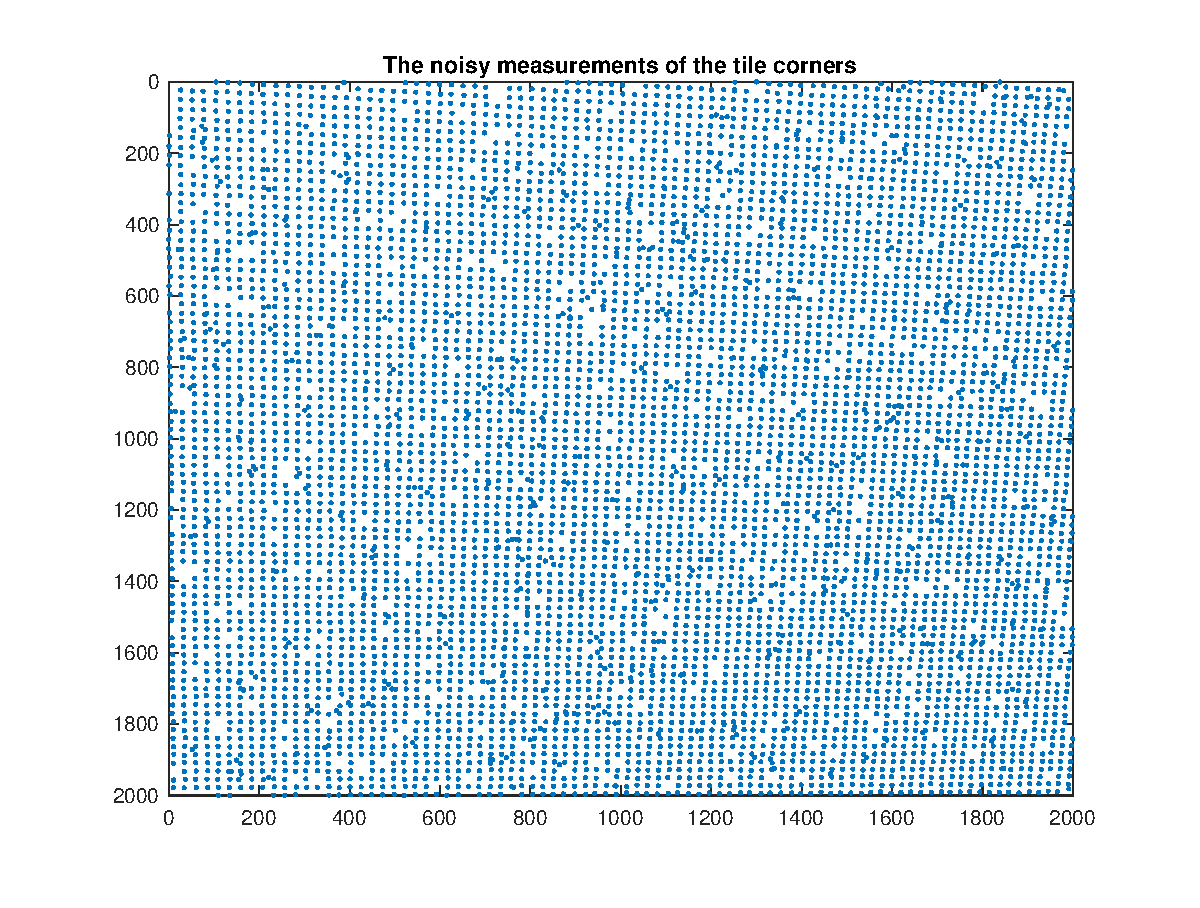
\includegraphics[width = 4.5cm, height=4.5cm]{GridImage.eps}
\end{figure}
%
We shall use to build our system of equations for an initial estimate of K-Matrix. insert fig 4 and say it is obtained by rearranging fig 3 above.
Our first minimisation task is finding the minimum norm solution of this system as there wont be an exact solution since estimates of image points will be noisy. (Discuss if the least square error i.e. the minimum norm of error is a good way to do this regression or not? Alternatives? Costs vs benefits?)
We use singular value decomposition (svd) to compute the inverse as that is more efficient for matlab to compute (look into expressing the cost difference between inv(A) and svd(A) functions in terms of big O notation?). Talk about the conditioning and its importance. Now we will have an estimate of the homography based on the 4 random points that we have chosen as known grid point and their correspondences.        
\subsubsection{Optimization}
Type of problem-convex etc.
Discussion about stopping criteria

\section{Overview of the Structure}
\subsection{Data Structure}
\subsection{Control Path}
\begin{wrapfigure}{r}{5.5cm}
\caption{Flowchart for the Estimation task involving RansSac}\label{wrap-fig:1}
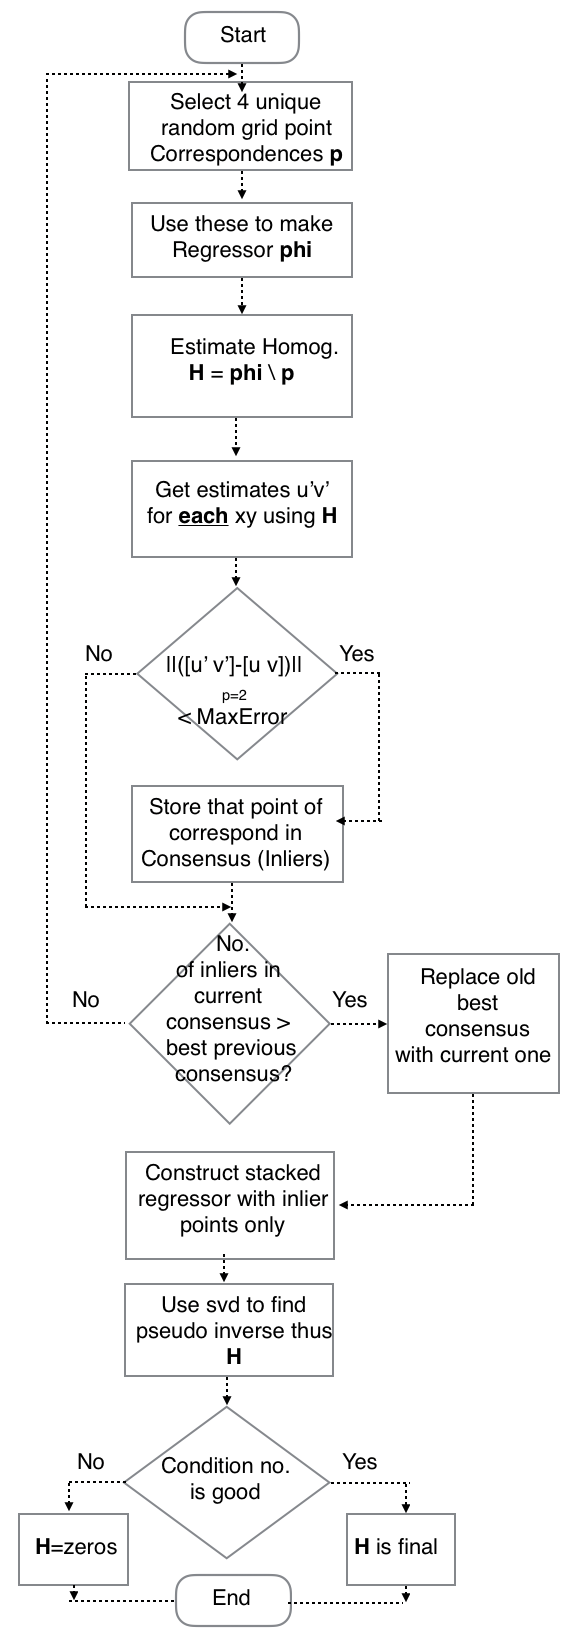
\includegraphics[width = 5.5cm, height=14cm]{Ransac_flowchart.png}
\end{wrapfigure} 
%------------------------------------------
BuildNoisyCorrespondences is my function that uses the position of the image and object (calibration grid or tsai tile) in world coordinates to calculate the image position of each grid corner in the pixel coordinates of the sensor plane. It uses the K-Matrix that we initially built using our manually set camera parameters. Now that we have a set of corresponding image coordinates for each corner on our tile (grid) we can choose randomly 4 points to construct our Regressor in fig 4. From the regressor we find our estimated homography. We use this homography to multiply with each and every point in the grid and find the error between the uv estimated using this homography and the uv we had found using the world coordinates position and initial K-Matrix. If this error is acceptable then we add this point into a Consensus set which is a set of inliers for our estimated parameters. We again choose randomly 4 known points and their correspondences and find another estimated homography and again compare the error given by our estimate with each and every point to obtain another consensus set. We do this process around 50 times and whichever time we have obtained the largest number of inliers we take the homography of that time to be our homograohy.

Least squares minimisation 

\section{Detailed Considerations}
\subsection{How to measure accuracy}
\begin{wrapfigure}{r}{5.5cm}
\caption{Varying number of RanSac runs vs accuracy of estimate.}\label{wrap-fig:1}
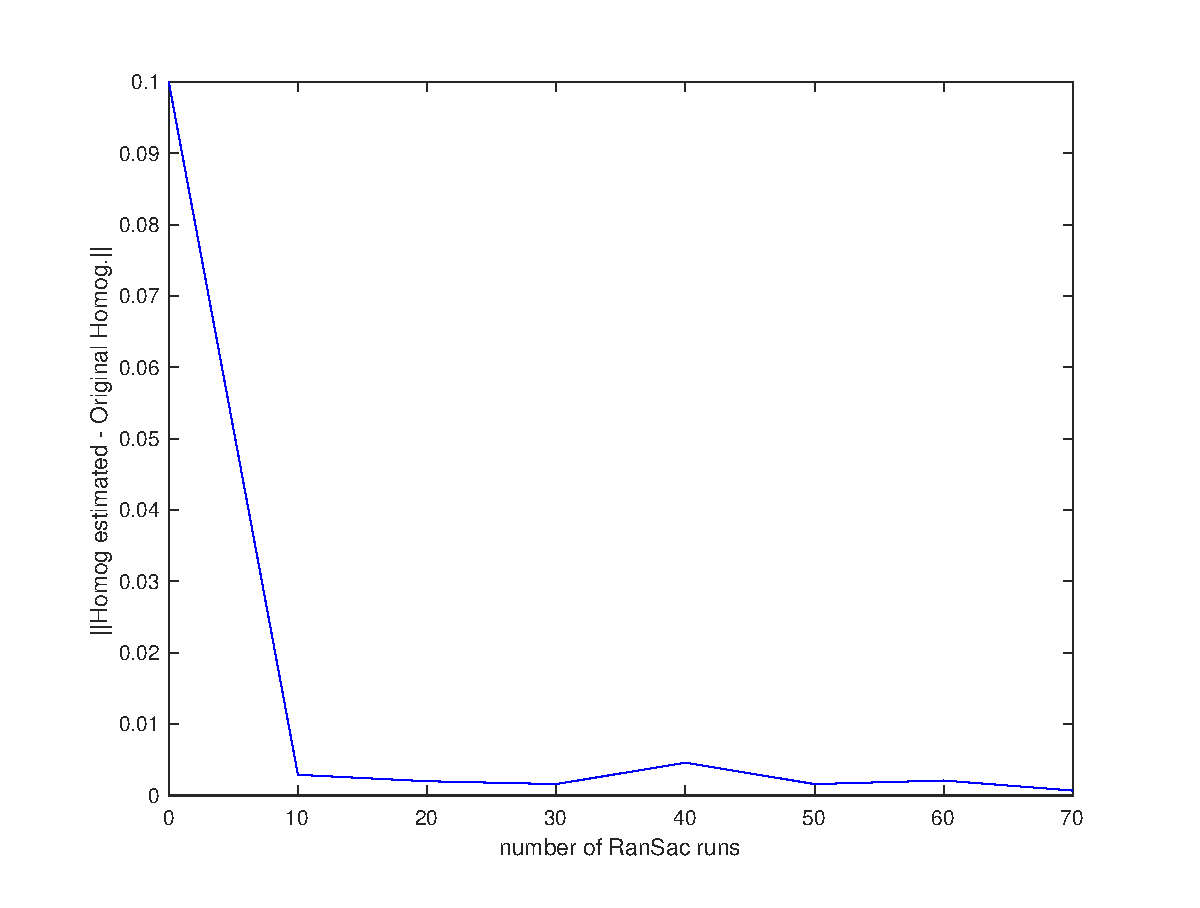
\includegraphics[width = 5.5cm, height=5.5cm]{HomogErrorVsRansacRuns.eps}
\end{wrapfigure} 



\begin{wrapfigure}{r}{5.5cm}
\caption{Varying MaxError acceptable for RanSac to consider point as inlier vs accuracy of estimate.}\label{wrap-fig:1}
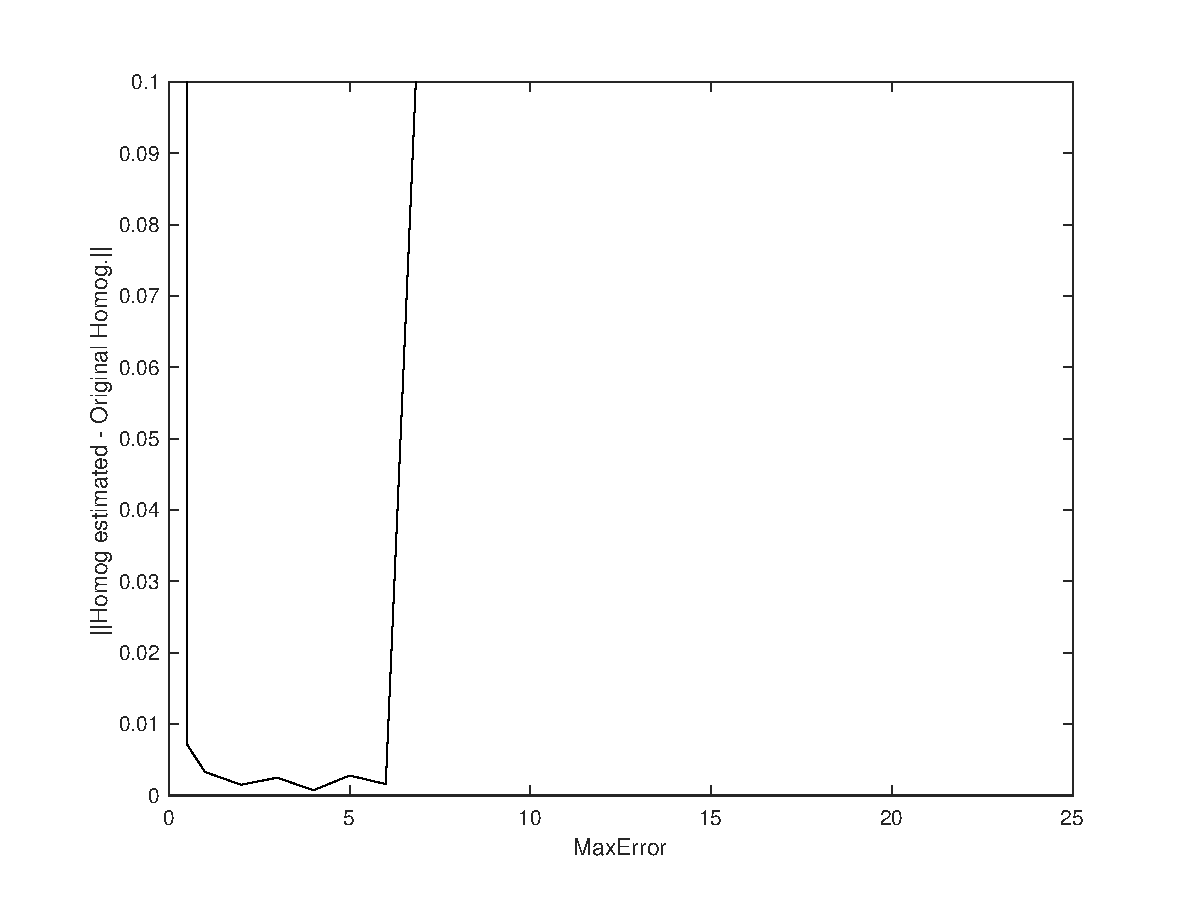
\includegraphics[width = 5.5cm, height=5.5cm]{MaxErrorVsHomogError.eps}
\end{wrapfigure} 

Analysis Fig2: Similar to fig 1 we are concerned with a general trend because of the randomness with which we choose our points each time despite the same parameters. More the ransac runs better is the estimate (lesser error) which is as one would expect because ransac will exclude outlier pixels and hence give us a better regressor to find homography from.

Similarly changing the MaxError value will have an effect on the accuracy of our estimate. Increasing the MaxError means we are increasing the threshold accuracy for an estimated uv to be part of consensus set. So we will have more strict inliers for higher MaxError hence more accuracy.

Analysis 3: Overfitting if the max error is too low as there will be very few points in the consensus hence the regressor for the robust inverse calculation will have too few points.

I have made the script also output how many elements are there in best consensus set for a given Max Error value and for an error of 1e-4 and a noise variance of .1 we just have 10 elements and this reduces if error is reduced or noise variance is increased. Too few points in consensus means when we use svd to find robust inverse and hence our Homography there are very few points and therefore a risk of overfitting. This can be seen in the poor accuracy ||Kestimated-Kmatrix|| for low Max Error in fig 3.

Other tests include: 
For zero noise and pOutlier = 0 K-Matrix estimated is the same as the K-Matrix and the BestConsensus set contains each and every grid point in the Correspond matrix. This is as expected because now all the points are “inliers” so ransac doesn't eliminate any points from the Consensus. This however isn't representative of the real world where we will encounter noisy images and some random points in our calibration image. 

\begin{wrapfigure}{r}{5.5cm}
\caption{Display of values stored inside Correspond. Number of columns represents total points on the grid (object).}\label{wrap-fig:1}
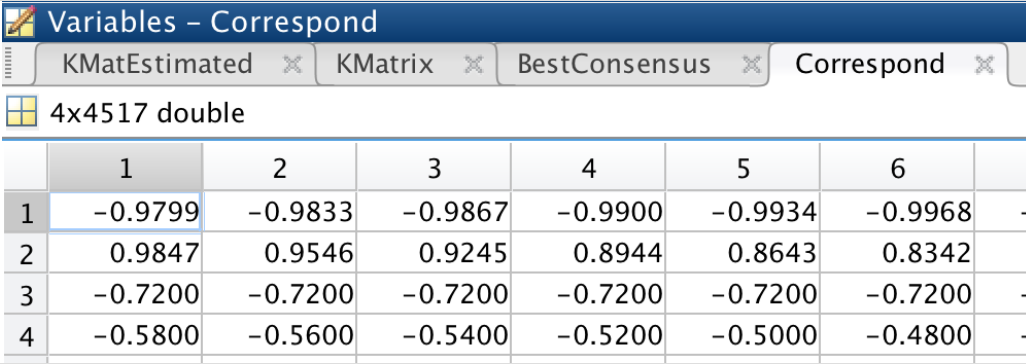
\includegraphics[width = 8.5cm, height=2.5cm]{Correspond_workspace.png}
\end{wrapfigure} 

\begin{wrapfigure}{r}{5.5cm}
\caption{The dimensions verify that BestConsensus vector contains all the points on the object i.e. no outliers when noise and pOutlier were set to zero.}\label{wrap-fig:1}
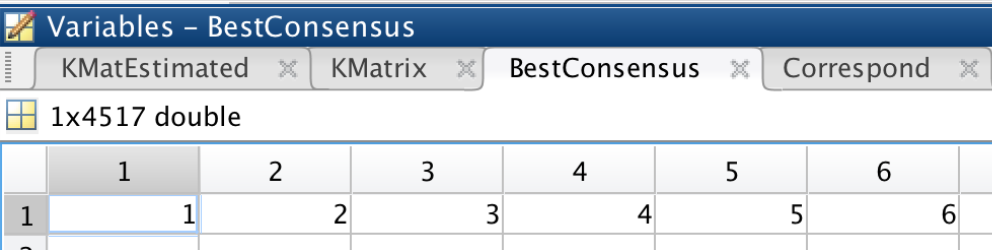
\includegraphics[width = 8.5cm, height=2.5cm]{BestConsensus_workspace.png}
\end{wrapfigure} 

Outputs and their tests with changing parameters
tests for ransack-consensus is same if no noise; homog=orighomog too
Test for svd try some unconditioned system you know of?
Norm of error between two K matrices? as an error metric

\subsection{Is this simulation a good model of the real world?}

Test final using real image
talk about finite diff vs analytic symbolic
using noise and outliers
While building up our correspondences we add noise to model the real world calibration tile where lets say some points appeared blurred due to slight camera motion. We try to mode white noise iid (?)
We also intentionally put in some outliers in these correspondences using a set probability to improve conditioning (how?).
Now if we set noise to zero 

Two methods to calculate the Jacobian were used to test a) if either one was implemented wrongly b) If the approximations used in the 1st method could be overcome by a more accurate 2nd method and thus provide us with an accurate optimisation solution.

The first method relied on using finite differences particularly forward difference estimate. The perturbation was set to .1 percent of the parameter and we used a for loop to manually differentiate with respect to each parameter and construct our blocks.

\section{Measures of Code Performance}
\subsection{Noise}
\begin{wrapfigure}{r}{5.5cm}
\caption{Effect of varying noise variance on accuracy of estimation.}\label{wrap-fig:1}
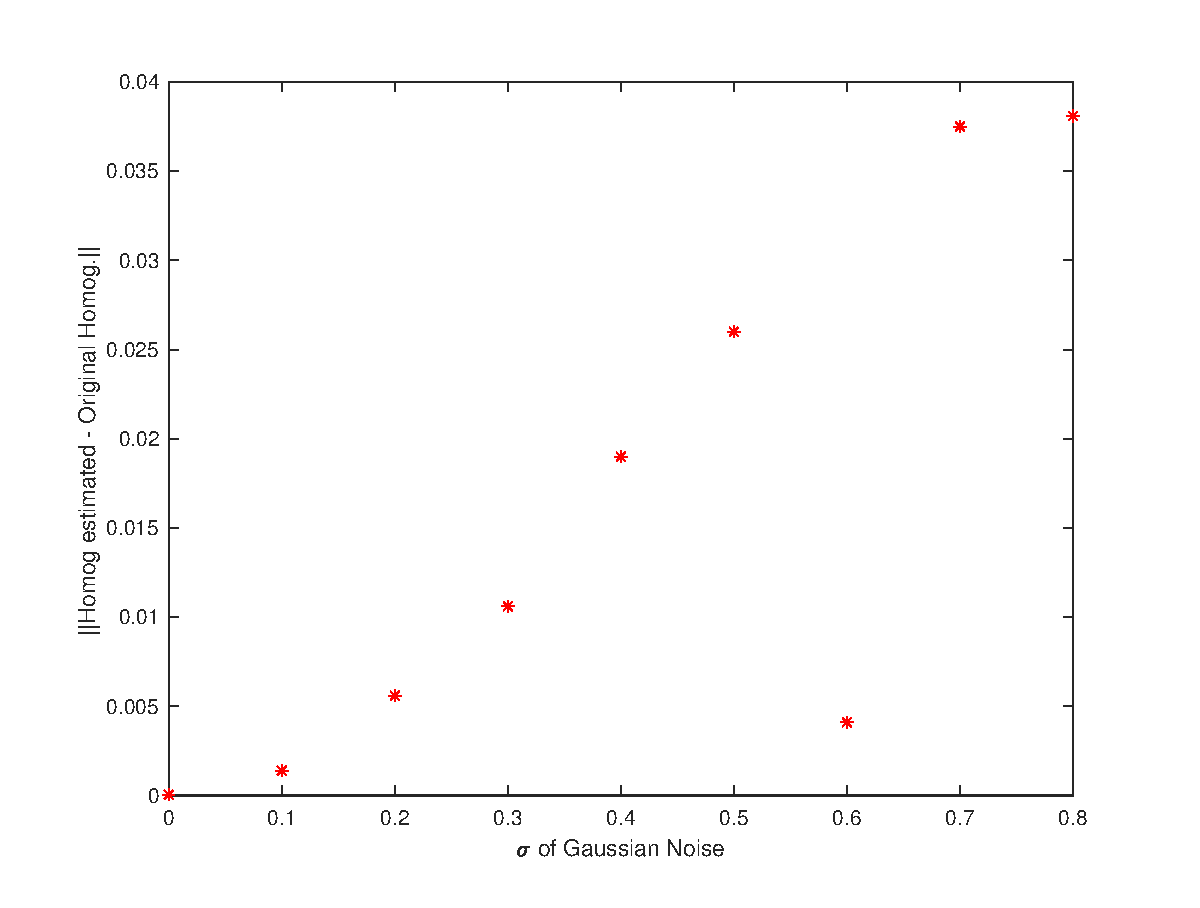
\includegraphics[width = 5.5cm, height=5.5cm]{HomogerrorVsNoiseVariance.eps}
\end{wrapfigure} 
Analysis: Fig 1: Trend is that more the noise variance I.e. the image pixels of calibration image are more apart from their true values then the worse the error between the Frobenius norm between true Homography matrix and the estimated. Although there is one outlier in the above trend, that is reasonable since we are randomly choosing points each time we run the estimate. So even with the same value of standard deviation and every other parameter, there will be variations in the error values which is why we can explain that as long as the trend is towards worse error with increased variance we can ignore this particular outlier in the above graph.

\subsection{Speed}
Maybe a table of threshold error to quit optim loop and time taken for each value?



\section{Conclusions}
\subsection{Assessment of Data Structures}
\subsection{How would I input real data?}
\subsection{How well did you do?}
Interestingly, results from both these methods were very similar and it was concluded that our forward difference approximation might suffice in this case. This served as a good test for verifying our algorithm for Jacobian.


However, the results we obtained were around a factor of 1000 off from our KMatEstimated. Even so, the optimisation loop was exited (hence the gradient was sufficiently low) which means that there is a strong possibility of the function to be stuck in a local minimum rather than the global minimum. Talk about the convex optimisation leading to global convergence etc. from notes and pawan’s email.


Maybe show 4 tables side by side showing the K-Matrix outputs -1. Original 2. Estimated 3. Optimized 4.using Jacobian and symbolic


\end{document}
